\documentclass{standalone}
\usepackage{tikz}
\usetikzlibrary{patterns, positioning}

\begin{document}
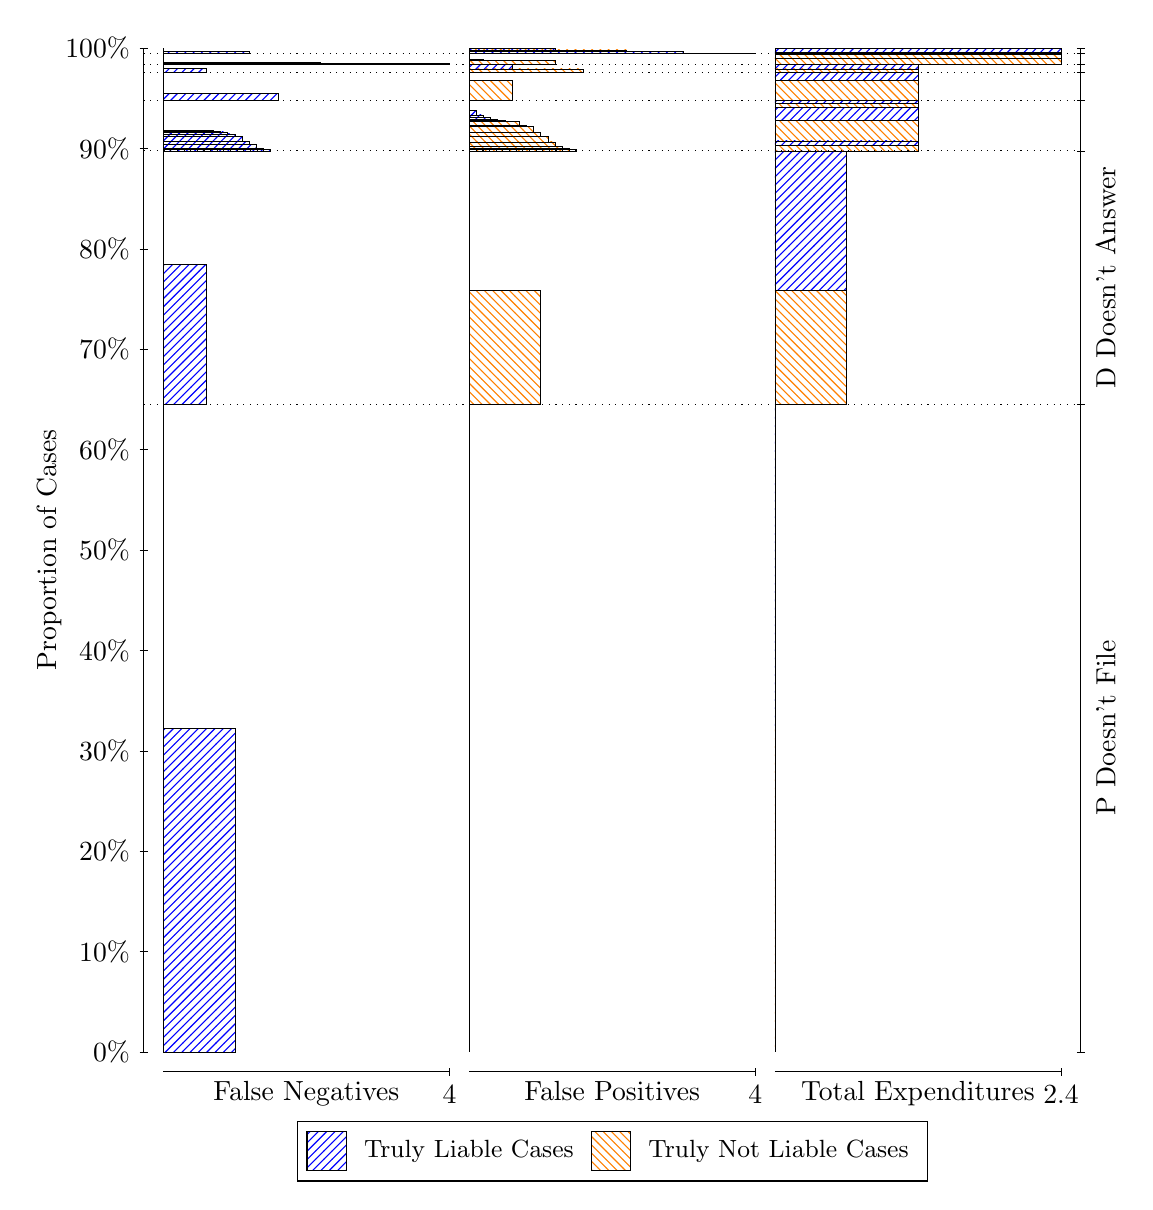
\begin{tikzpicture}
\draw[black, very thin] (1.5,1.75) -- (1.5,14.5);
\node[rotate=90, anchor=center] at (0.3, 8.125) {Proportion of Cases};
\draw[black, very thin] (1.45,1.75) -- (1.55,1.75);
\node[anchor=east] at (1.45, 1.75) {0\%};
\draw[black, very thin] (1.45,3.025) -- (1.55,3.025);
\node[anchor=east] at (1.45, 3.025) {10\%};
\draw[black, very thin] (1.45,4.3) -- (1.55,4.3);
\node[anchor=east] at (1.45, 4.3) {20\%};
\draw[black, very thin] (1.45,5.575) -- (1.55,5.575);
\node[anchor=east] at (1.45, 5.575) {30\%};
\draw[black, very thin] (1.45,6.85) -- (1.55,6.85);
\node[anchor=east] at (1.45, 6.85) {40\%};
\draw[black, very thin] (1.45,8.125) -- (1.55,8.125);
\node[anchor=east] at (1.45, 8.125) {50\%};
\draw[black, very thin] (1.45,9.4) -- (1.55,9.4);
\node[anchor=east] at (1.45, 9.4) {60\%};
\draw[black, very thin] (1.45,10.675) -- (1.55,10.675);
\node[anchor=east] at (1.45, 10.675) {70\%};
\draw[black, very thin] (1.45,11.95) -- (1.55,11.95);
\node[anchor=east] at (1.45, 11.95) {80\%};
\draw[black, very thin] (1.45,13.225) -- (1.55,13.225);
\node[anchor=east] at (1.45, 13.225) {90\%};
\draw[black, very thin] (1.45,14.5) -- (1.55,14.5);
\node[anchor=east] at (1.45, 14.5) {100\%};

\draw[black, very thin] (13.4,1.75) -- (13.4,14.5);
\draw[black, very thin] (13.35,1.75) -- (13.45,1.75);
\node[anchor=west] at (13.35, 1.75) {};
\draw[black, very thin] (13.35,9.9781) -- (13.45,9.9781);
\node[anchor=west] at (13.35, 9.9781) {};
\draw[black, very thin] (13.35,13.194) -- (13.45,13.194);
\node[anchor=west] at (13.35, 13.194) {};
\draw[black, very thin] (13.35,13.832) -- (13.45,13.832);
\node[anchor=west] at (13.35, 13.832) {};
\draw[black, very thin] (13.35,14.186) -- (13.45,14.186);
\node[anchor=west] at (13.35, 14.186) {};
\draw[black, very thin] (13.35,14.295) -- (13.45,14.295);
\node[anchor=west] at (13.35, 14.295) {};
\draw[black, very thin] (13.35,14.43) -- (13.45,14.43);
\node[anchor=west] at (13.35, 14.43) {};
\draw[black, very thin] (13.35,14.5) -- (13.45,14.5);
\node[anchor=west] at (13.35, 14.5) {};

\draw[black, very thin, pattern color=blue, pattern=north east lines] (1.75,1.75) rectangle (2.6583,5.864);
\draw[black, very thin, pattern color=orange, pattern=north west lines] (1.75,5.864) rectangle (1.75,9.9781);
\draw[black, very thin, pattern color=blue, pattern=north east lines] (1.75,9.9781) rectangle (2.295,11.754);
\draw[black, very thin, pattern color=orange, pattern=north west lines] (1.75,11.754) rectangle (1.75,13.194);
\draw[black, very thin, pattern color=blue, pattern=north east lines] (1.75,13.194) rectangle (3.1125,13.216);
\draw[black, very thin, pattern color=blue, pattern=north east lines] (1.75,13.216) rectangle (3.0217,13.229);
\draw[black, very thin, pattern color=blue, pattern=north east lines] (1.75,13.229) rectangle (2.9308,13.274);
\draw[black, very thin, pattern color=blue, pattern=north east lines] (1.75,13.274) rectangle (2.84,13.316);
\draw[black, very thin, pattern color=blue, pattern=north east lines] (1.75,13.316) rectangle (2.7492,13.375);
\draw[black, very thin, pattern color=blue, pattern=north east lines] (1.75,13.375) rectangle (2.6583,13.409);
\draw[black, very thin, pattern color=blue, pattern=north east lines] (1.75,13.409) rectangle (2.5675,13.436);
\draw[black, very thin, pattern color=blue, pattern=north east lines] (1.75,13.436) rectangle (2.4767,13.445);
\draw[black, very thin, pattern color=blue, pattern=north east lines] (1.75,13.445) rectangle (2.3858,13.455);
\draw[black, very thin, pattern color=orange, pattern=north west lines] (1.75,13.455) rectangle (1.75,13.832);
\draw[black, very thin, pattern color=blue, pattern=north east lines] (1.75,13.832) rectangle (3.2033,13.927);
\draw[black, very thin, pattern color=orange, pattern=north west lines] (1.75,13.927) rectangle (1.75,14.186);
\draw[black, very thin, pattern color=blue, pattern=north east lines] (1.75,14.186) rectangle (2.295,14.245);
\draw[black, very thin, pattern color=orange, pattern=north west lines] (1.75,14.245) rectangle (1.75,14.295);
\draw[black, very thin, pattern color=blue, pattern=north east lines] (1.75,14.295) rectangle (5.3833,14.301);
\draw[black, very thin, pattern color=blue, pattern=north east lines] (1.75,14.301) rectangle (3.7483,14.314);
\draw[black, very thin, pattern color=orange, pattern=north west lines] (1.75,14.314) rectangle (1.75,14.43);
\draw[black, very thin, pattern color=blue, pattern=north east lines] (1.75,14.43) rectangle (2.84,14.453);
\draw[black, very thin, pattern color=orange, pattern=north west lines] (1.75,14.453) rectangle (1.75,14.472);
\draw[black, very thin, pattern color=blue, pattern=north east lines] (1.75,14.472) rectangle (1.75,14.5);
\draw[black, very thin, pattern color=orange, pattern=north west lines] (5.6333,1.75) rectangle (5.6333,5.8641);
\draw[black, very thin, pattern color=blue, pattern=north east lines] (5.6333,5.8641) rectangle (5.6333,9.9781);
\draw[black, very thin, pattern color=orange, pattern=north west lines] (5.6333,9.9781) rectangle (6.5417,11.418);
\draw[black, very thin, pattern color=blue, pattern=north east lines] (5.6333,11.418) rectangle (5.6333,13.194);
\draw[black, very thin, pattern color=orange, pattern=north west lines] (5.6333,13.194) rectangle (6.9958,13.208);
\draw[black, very thin, pattern color=orange, pattern=north west lines] (5.6333,13.208) rectangle (6.905,13.222);
\draw[black, very thin, pattern color=orange, pattern=north west lines] (5.6333,13.222) rectangle (6.8142,13.254);
\draw[black, very thin, pattern color=orange, pattern=north west lines] (5.6333,13.254) rectangle (6.7233,13.309);
\draw[black, very thin, pattern color=orange, pattern=north west lines] (5.6333,13.309) rectangle (6.6325,13.378);
\draw[black, very thin, pattern color=orange, pattern=north west lines] (5.6333,13.378) rectangle (6.5417,13.429);
\draw[black, very thin, pattern color=orange, pattern=north west lines] (5.6333,13.429) rectangle (6.4508,13.5);
\draw[black, very thin, pattern color=orange, pattern=north west lines] (5.6333,13.5) rectangle (6.36,13.52);
\draw[black, very thin, pattern color=orange, pattern=north west lines] (5.6333,13.52) rectangle (6.2692,13.572);
\draw[black, very thin, pattern color=blue, pattern=north east lines] (5.6333,13.572) rectangle (6.0875,13.581);
\draw[black, very thin, pattern color=blue, pattern=north east lines] (5.6333,13.581) rectangle (5.9967,13.591);
\draw[black, very thin, pattern color=blue, pattern=north east lines] (5.6333,13.591) rectangle (5.9058,13.617);
\draw[black, very thin, pattern color=blue, pattern=north east lines] (5.6333,13.617) rectangle (5.815,13.652);
\draw[black, very thin, pattern color=blue, pattern=north east lines] (5.6333,13.652) rectangle (5.7242,13.711);
\draw[black, very thin, pattern color=blue, pattern=north east lines] (5.6333,13.711) rectangle (5.6333,13.832);
\draw[black, very thin, pattern color=orange, pattern=north west lines] (5.6333,13.832) rectangle (6.1783,14.091);
\draw[black, very thin, pattern color=blue, pattern=north east lines] (5.6333,14.091) rectangle (5.6333,14.186);
\draw[black, very thin, pattern color=orange, pattern=north west lines] (5.6333,14.186) rectangle (7.0867,14.236);
\draw[black, very thin, pattern color=blue, pattern=north east lines] (5.6333,14.236) rectangle (6.1783,14.295);
\draw[black, very thin, pattern color=orange, pattern=north west lines] (5.6333,14.295) rectangle (6.7233,14.341);
\draw[black, very thin, pattern color=blue, pattern=north east lines] (5.6333,14.341) rectangle (5.815,14.354);
\draw[black, very thin, pattern color=orange, pattern=north west lines] (5.6333,14.354) rectangle (5.6333,14.424);
\draw[black, very thin, pattern color=blue, pattern=north east lines] (5.6333,14.424) rectangle (5.6333,14.43);
\draw[black, very thin, pattern color=orange, pattern=north west lines] (5.6333,14.43) rectangle (9.2667,14.434);
\draw[black, very thin, pattern color=blue, pattern=north east lines] (5.6333,14.434) rectangle (8.3583,14.462);
\draw[black, very thin, pattern color=orange, pattern=north west lines] (5.6333,14.462) rectangle (7.6317,14.477);
\draw[black, very thin, pattern color=blue, pattern=north east lines] (5.6333,14.477) rectangle (6.7233,14.5);
\draw[black, very thin, pattern color=orange, pattern=north west lines] (9.5167,1.75) rectangle (9.5167,5.8641);
\draw[black, very thin, pattern color=blue, pattern=north east lines] (9.5167,5.8641) rectangle (9.5167,9.9781);
\draw[black, very thin, pattern color=orange, pattern=north west lines] (9.5167,9.9781) rectangle (10.425,11.418);
\draw[black, very thin, pattern color=blue, pattern=north east lines] (9.5167,11.418) rectangle (10.425,13.194);
\draw[black, very thin, pattern color=orange, pattern=north west lines] (9.5167,13.194) rectangle (11.333,13.263);
\draw[black, very thin, pattern color=blue, pattern=north east lines] (9.5167,13.263) rectangle (11.333,13.322);
\draw[black, very thin, pattern color=orange, pattern=north west lines] (9.5167,13.322) rectangle (11.333,13.584);
\draw[black, very thin, pattern color=blue, pattern=north east lines] (9.5167,13.584) rectangle (11.333,13.75);
\draw[black, very thin, pattern color=orange, pattern=north west lines] (9.5167,13.75) rectangle (11.333,13.796);
\draw[black, very thin, pattern color=blue, pattern=north east lines] (9.5167,13.796) rectangle (11.333,13.832);
\draw[black, very thin, pattern color=orange, pattern=north west lines] (9.5167,13.832) rectangle (11.333,14.091);
\draw[black, very thin, pattern color=blue, pattern=north east lines] (9.5167,14.091) rectangle (11.333,14.186);
\draw[black, very thin, pattern color=orange, pattern=north west lines] (9.5167,14.186) rectangle (11.333,14.236);
\draw[black, very thin, pattern color=blue, pattern=north east lines] (9.5167,14.236) rectangle (11.333,14.295);
\draw[black, very thin, pattern color=orange, pattern=north west lines] (9.5167,14.295) rectangle (13.15,14.364);
\draw[black, very thin, pattern color=blue, pattern=north east lines] (9.5167,14.364) rectangle (13.15,14.37);
\draw[black, very thin, pattern color=orange, pattern=north west lines] (9.5167,14.37) rectangle (13.15,14.417);
\draw[black, very thin, pattern color=blue, pattern=north east lines] (9.5167,14.417) rectangle (13.15,14.43);
\draw[black, very thin, pattern color=orange, pattern=north west lines] (9.5167,14.43) rectangle (13.15,14.449);
\draw[black, very thin, pattern color=blue, pattern=north east lines] (9.5167,14.449) rectangle (13.15,14.5);
\draw[black, dotted] (1.5,9.9781) -- (13.4,9.9781);
\draw[black, dotted] (1.5,13.194) -- (13.4,13.194);
\draw[black, dotted] (1.5,13.832) -- (13.4,13.832);
\draw[black, dotted] (1.5,14.186) -- (13.4,14.186);
\draw[black, dotted] (1.5,14.295) -- (13.4,14.295);
\draw[black, dotted] (1.5,14.43) -- (13.4,14.43);
\draw[black, very thin] (1.75,1.5) -- (5.3833,1.5);
\node[anchor=north] at (3.5667, 1.5) {False Negatives};
\draw[black, very thin] (5.3833,1.45) -- (5.3833,1.55);
\node[anchor=north] at (5.3833, 1.45) {4};

\draw[black, very thin] (5.6333,1.5) -- (9.2667,1.5);
\node[anchor=north] at (7.45, 1.5) {False Positives};
\draw[black, very thin] (9.2667,1.45) -- (9.2667,1.55);
\node[anchor=north] at (9.2667, 1.45) {4};

\draw[black, very thin] (9.5167,1.5) -- (13.15,1.5);
\node[anchor=north] at (11.333, 1.5) {Total Expenditures};
\draw[black, very thin] (13.15,1.45) -- (13.15,1.55);
\node[anchor=north] at (13.15, 1.45) {2.4};

\node[black, centered, rotate=90] at (13.72, 5.8641) {P Doesn't File};
\node[black, centered, rotate=90] at (13.72, 11.586) {D Doesn't Answer};






\draw (7.449999999999999,1.5) node[draw=none] (baseCoordinate) {};
\begin{scope}[align=center]
        \matrix[scale=0.5, draw=black, below=0.5cm of baseCoordinate, nodes={draw}, column sep=0.1cm]{
            \node[rectangle, draw, minimum width=0.5cm, minimum height=0.5cm, pattern=north east lines, pattern color=blue] {}; &
            \node[draw=none, font=\small] (B) {Truly Liable Cases}; &
            \node[rectangle, draw, minimum width=0.5cm, minimum height=0.5cm, pattern=north west lines, pattern color=orange] {}; &
            \node[draw=none, font=\small] (B) {Truly Not Liable Cases}; \\
            };
\end{scope}

\end{tikzpicture}
\end{document}